%======================================================================
\section{Esquemático completo}\label{ap:esquema}
%======================================================================
As folhas do esquemático da PCB v1, na ordem do arquivo do KiCad, recortadas no circuito
(sem a moldura e o carimbo). A folha principal está na Figura~\ref{fig:esquema_raiz}; o arquivo
completo, em PDF, fica em \code{hardware/placas/v1/esquema.pdf}.

\begin{figure}[H]
\centering
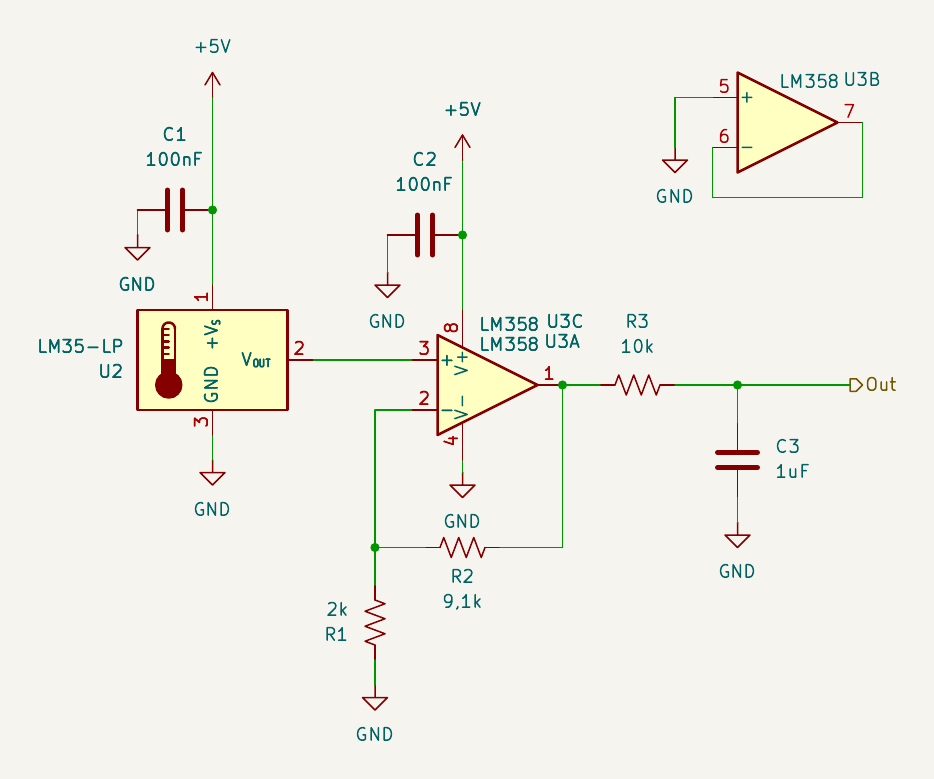
\includegraphics[scale=1.3]{figuras/esquema_p2.png}
\caption{Folha do LM35: sensor, LM358 (as duas metades) e filtro RC.}
\end{figure}

\begin{figure}[H]
\centering
\begin{subfigure}[b]{0.56\linewidth}
  \centering
  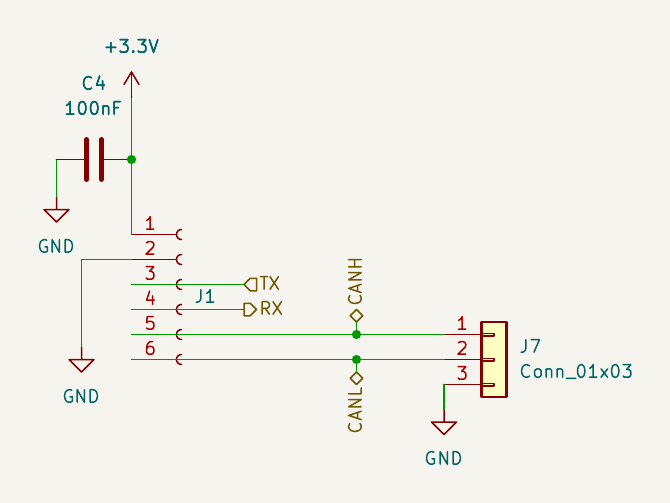
\includegraphics[scale=1.3]{figuras/esquema_p3.png}
  \caption{CAN: módulo transceptor (J1) e conector do barramento (J7).}
\end{subfigure}\hfill
\begin{subfigure}[b]{0.40\linewidth}
  \centering
  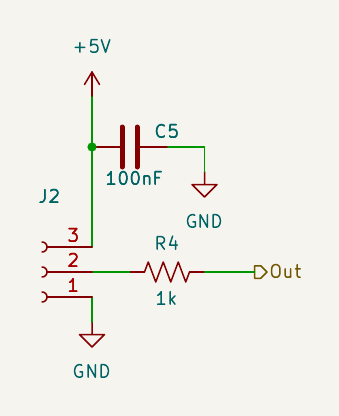
\includegraphics[scale=1.3]{figuras/esquema_p4.png}
  \caption{PIR HC-SR501 (J2), com R4 em série.}
\end{subfigure}
\caption{Folhas do CAN e do PIR.}
\end{figure}

\begin{figure}[H]
\centering
\begin{subfigure}[b]{0.24\linewidth}
  \centering
  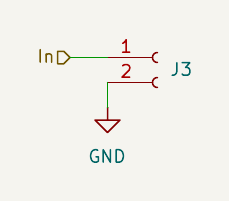
\includegraphics[scale=1.3]{figuras/esquema_p5.png}
  \caption{Porta 1 (J3).}
\end{subfigure}\hfill
\begin{subfigure}[b]{0.24\linewidth}
  \centering
  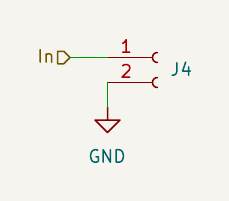
\includegraphics[scale=1.3]{figuras/esquema_p6.png}
  \caption{Porta 2 (J4).}
\end{subfigure}\hfill
\begin{subfigure}[b]{0.40\linewidth}
  \centering
  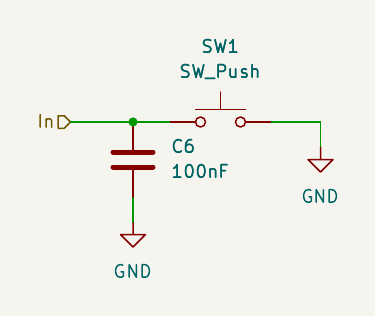
\includegraphics[scale=1.3]{figuras/esquema_p7.png}
  \caption{Botão da pulseira (SW1).}
\end{subfigure}

\vspace{4mm}
\begin{subfigure}[b]{0.40\linewidth}
  \centering
  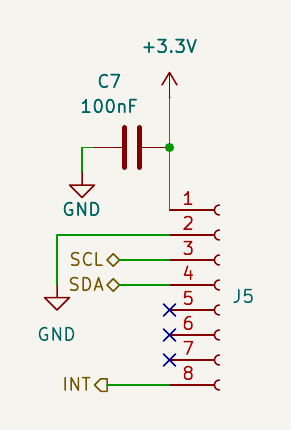
\includegraphics[scale=1.3]{figuras/esquema_p8.png}
  \caption{MPU-6050 (J5).}
\end{subfigure}\hfill
\begin{subfigure}[b]{0.40\linewidth}
  \centering
  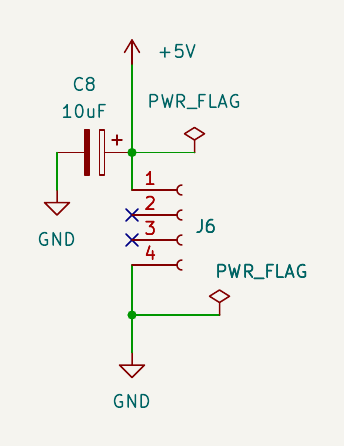
\includegraphics[scale=1.3]{figuras/esquema_p9.png}
  \caption{Entrada USB-C (J6).}
\end{subfigure}
\caption{Folhas das portas, do botão, do MPU-6050 e da alimentação.}
\end{figure}

%======================================================================
\section{Mapa de pinos completo}\label{ap:pinos}
%======================================================================
\begin{table}[H]
\centering
\caption{Mapa de pinos da PCB v1 (\code{firmware/common/pcb/include/pcb\_pins.h}).}
\label{tab:pinos_completo}
\small
\begin{tabular}{@{}l>{\raggedright\arraybackslash}p{5.0cm}l>{\raggedright\arraybackslash}p{5.2cm}@{}}
\toprule
GPIO & Função & Placa & Observação \\
\midrule
1 & I²C SDA (MPU-6050) & pulseira & par do ULP; ADC1, canal 0, usado como digital \\
2 & I²C SCL & pulseira & par do ULP; ADC1, canal 1 \\
4 & LM35 (saída do LM358) & hub & ADC1, canal 3 \\
5 & reservado: bateria de uma pulseira própria & --- & ADC1, canal 4; sem divisor nesta PCB \\
6, 7 & reserva analógica & --- & ADC1, canais 5 e 6 \\
8 & PIR HC-SR501 & hub & ADC1, canal 7, usado como digital \\
9, 10 & portas 3 e 4 (opcionais) & hub & ADC1, canais 8 e 9 \\
11, 12 & portas 1 (quarto) e 2 (banheiro) & hub & ADC2, mas digitais \\
13, 14 & CAN TX e RX & os dois & na pulseira, só em bancada \\
15, 16 & não ligar: cristal de 32\,kHz & --- & reserva \\
17 & interrupção do MPU-6050 & pulseira & RTC GPIO \\
18 & botão da pulseira & pulseira & RTC GPIO; \textit{pull-up} interno e filtro de \textit{glitch} \\
21 & livre (era o buzzer) & --- & \\
38 ou 48 & LED WS2812 & os dois & o da DevKit (v1.1 ou v1.0), escolhido no \code{menuconfig} \\
39--42 & expansão (por exemplo, portas 5 a 8) & --- & só enquanto o JTAG por pinos não for usado \\
\bottomrule
\end{tabular}
\end{table}

Para acrescentar uma porta, basta uma linha na tabela \code{BOARD\_DOORS} do hub: o firmware
cria a entrada, o tópico \code{porta/<id>} e o identificador CAN. São até 8 portas, uma por
identificador (\code{0x0F3} a \code{0x0FA}); o build falha se passar disso.

%======================================================================
\section{Lista de materiais e custo}\label{ap:bom}
%======================================================================
\begin{table}[H]
\centering
\caption{Lista de materiais da PCB v1 (gerada do KiCad).}
\label{tab:bom}
\footnotesize
% Gerado por modelo/experimentos/12_relatorio_q2.py a partir de hardware/placas/v1/lista-de-materiais.csv
\begin{tabular}{@{}l >{\raggedright\arraybackslash}p{2.3cm} >{\raggedright\arraybackslash}p{4.4cm} >{\raggedright\arraybackslash}p{4.4cm} r@{}}
\toprule
Referência & Valor & Função & Footprint & Qtd \\
\midrule
C1,C2,C4-C7 & 100\,nF & desacoplamento (LM35, LM358, CAN, PIR, botão, MPU) & \texttt{\scriptsize C\_\allowbreak{}Disc\_\allowbreak{}D3.0mm\_\allowbreak{}W1.6mm\_\allowbreak{}P2.50mm} & 6 \\
C3 & 1\,µF & filtro RC na entrada do ADC (com R3) & \texttt{\scriptsize C\_\allowbreak{}Rect\_\allowbreak{}L4.0mm\_\allowbreak{}W2.5mm\_\allowbreak{}P2.50mm} & 1 \\
C8 & 10\,µF & reservatório na entrada de 5 V & \texttt{\scriptsize CP\_\allowbreak{}Radial\_\allowbreak{}D5.0mm\_\allowbreak{}P2.00mm} & 1 \\
D1 & 1N5819 & impede juntar duas fontes no 5 V da DevKit & \texttt{\scriptsize D\_\allowbreak{}DO-41\_\allowbreak{}SOD81\_\allowbreak{}P10.16mm\_\allowbreak{}Horizontal} & 1 \\
J1 & Conn\_\allowbreak{}01x06\_\allowbreak{}Socket & módulo transceptor CAN SN65HVD230 & \texttt{\scriptsize WCMCU-230} & 1 \\
J2 & Conn\_\allowbreak{}01x03\_\allowbreak{}Socket & módulo PIR HC-SR501 & \texttt{\scriptsize HCSR501} & 1 \\
J3,J4 & Conn\_\allowbreak{}01x02\_\allowbreak{}Socket & portas 1 e 2 (reed MC-38) & \texttt{\scriptsize PinSocket\_\allowbreak{}1x02\_\allowbreak{}P2.54mm\_\allowbreak{}Vertical} & 2 \\
J5 & Conn\_\allowbreak{}01x08\_\allowbreak{}Socket & módulo MPU-6050 (GY-521) & \texttt{\scriptsize MPU6050} & 1 \\
J6 & Conn\_\allowbreak{}01x04\_\allowbreak{}Socket & módulo USB-C (entrada de 5 V) & \texttt{\scriptsize Modulo USB-C} & 1 \\
J7 & Conn\_\allowbreak{}01x03 & barramento CAN (CANH, CANL, GND) & \texttt{\scriptsize PinHeader\_\allowbreak{}1x03\_\allowbreak{}P2.54mm\_\allowbreak{}Vertical} & 1 \\
R1 & 2k & ganho do LM358 (para o GND) & \texttt{\scriptsize R\_\allowbreak{}Axial\_\allowbreak{}DIN0207\_\allowbreak{}L6.3mm\_\allowbreak{}D2.5mm\_\allowbreak{}P10.16mm\_\allowbreak{}Horizontal} & 1 \\
R2 & 9,1k & ganho do LM358 (realimentação) & \texttt{\scriptsize R\_\allowbreak{}Axial\_\allowbreak{}DIN0207\_\allowbreak{}L6.3mm\_\allowbreak{}D2.5mm\_\allowbreak{}P10.16mm\_\allowbreak{}Horizontal} & 1 \\
R3 & 10k & filtro RC (com C3) & \texttt{\scriptsize R\_\allowbreak{}Axial\_\allowbreak{}DIN0207\_\allowbreak{}L6.3mm\_\allowbreak{}D2.5mm\_\allowbreak{}P10.16mm\_\allowbreak{}Horizontal} & 1 \\
R4 & 1k & série na saída do PIR & \texttt{\scriptsize R\_\allowbreak{}Axial\_\allowbreak{}DIN0207\_\allowbreak{}L6.3mm\_\allowbreak{}D2.5mm\_\allowbreak{}P10.16mm\_\allowbreak{}Horizontal} & 1 \\
SW1 & SW\_\allowbreak{}Push & botão ``estou bem'' & \texttt{\scriptsize SW\_\allowbreak{}PUSH-12mm} & 1 \\
TP1 & 5V & ponto de teste & \texttt{\scriptsize TestPoint\_\allowbreak{}Pad\_\allowbreak{}D1.5mm} & 1 \\
TP2 & 3V3 & ponto de teste & \texttt{\scriptsize TestPoint\_\allowbreak{}Pad\_\allowbreak{}D1.5mm} & 1 \\
TP3 & GND & ponto de teste & \texttt{\scriptsize TestPoint\_\allowbreak{}Pad\_\allowbreak{}D1.5mm} & 1 \\
TP4 & LM35 & ponto de teste (saída do LM358) & \texttt{\scriptsize TestPoint\_\allowbreak{}Pad\_\allowbreak{}D1.5mm} & 1 \\
TP5 & CANH & ponto de teste & \texttt{\scriptsize TestPoint\_\allowbreak{}Pad\_\allowbreak{}D1.5mm} & 1 \\
TP6 & CANL & ponto de teste & \texttt{\scriptsize TestPoint\_\allowbreak{}Pad\_\allowbreak{}D1.5mm} & 1 \\
U1 & ESP32-S3-DevKitC & ESP32-S3-DevKitC-1 encaixada & \texttt{\scriptsize ESP32-S3-DevKitC} & 1 \\
U2 & LM35-LP & sensor de temperatura LM35DZ & \texttt{\scriptsize TO-92\_\allowbreak{}Inline\_\allowbreak{}Wide} & 1 \\
U3 & LM358 & amp-op LM358 (soquete DIP-8) & \texttt{\scriptsize DIP-8\_\allowbreak{}W7.62mm\_\allowbreak{}Socket\_\allowbreak{}LongPads} & 1 \\
\midrule
\multicolumn{4}{@{}l}{Total} & 30 \\
\bottomrule
\end{tabular}

\end{table}

Além das peças da placa: a ESP32-S3-DevKitC-1, os módulos HC-SR501, GY-521 (MPU-6050),
WCMCU-230 (SN65HVD230) e USB-C, os reed switches MC-38 com fio até as portas e, por placa, um
carregador USB-A ou um \textit{power bank} com cabo USB-A $\to$ C.

\subsection*{Custo item por item}

A Tabela~\ref{tab:custo} detalha o custo de um quarto, resumido na Seção~\ref{sec:custo}: o hub
e a pulseira, cada um numa PCB v1 só com as peças da sua função, mais os sensores de porta, a
alimentação e as caixas.

Os preços são do varejo brasileiro, por unidade, consultados nos sites das lojas em
\custoData{}, sem frete; os links estão em \code{hardware/placas/v1/custo-estimado.csv}. Uma
peça vendida em pacote entra pelo preço de uma unidade. Duas linhas são estimativas
($\approx$). Uma é o capacitor de poliéster. A outra é a PCB: a JLCPCB cobra US\$\,2 pelas cinco
placas, mas o frete até o Brasil e os impostos só aparecem no pedido. A conta usa frete de cerca
de US\$\,15, 60\,\% de imposto de importação, 20\,\% de ICMS e R\$\,5,15 por dólar. No
protótipo, a pulseira é a mesma placa de $100 \times 60$\,mm, numa caixa igual à do hub.

\begin{table}[H]
\centering
\caption{Custo estimado do kit de um quarto (hub e pulseira), em reais.}
\label{tab:custo}
\footnotesize
% Gerado por modelo/experimentos/12_relatorio_q2.py a partir de hardware/placas/v1/custo-estimado.csv
\begin{tabularx}{\linewidth}{@{}>{\raggedright\arraybackslash}X c c r r l@{}}
\toprule
Item & Hub & Pulseira & R\$ unit. & R\$ no kit & Loja \\
\midrule
\multicolumn{6}{@{}l}{\textit{Placa e módulos}} \\
PCB v1 (1/5 do pedido de 5 placas) & 1 & 1 & $\approx$\,35,00 & 70,00 & JLCPCB \\
ESP32-S3-DevKitC-1 N16R8 & 1 & 1 & 94,30 & 188,60 & Curto Circuito \\
Módulo PIR HC-SR501 & 1 & --- & 11,90 & 11,90 & Eletrogate \\
Módulo CAN SN65HVD230 & 1 & --- & 10,90 & 10,90 & Smart Kits \\
Sensor magnético de porta MC-38 & 2 & --- & 7,90 & 15,80 & Eletrogate \\
Cabo até as portas (rolo de 5 m) & 2 & --- & 9,46 & 18,92 & Usinainfo \\
Módulo MPU-6050 (GY-521) & --- & 1 & 19,90 & 19,90 & Eletrogate \\
Módulo USB-C fêmea para DIP & 1 & 1 & 2,90 & 5,80 & AutoCore Robótica \\
\multicolumn{6}{@{}l}{\textit{Componentes}} \\
Sensor de temperatura LM35DZ & 1 & --- & 10,90 & 10,90 & Eletrogate \\
Amplificador operacional LM358P & 1 & --- & 1,50 & 1,50 & AutoCore Robótica \\
Soquete DIP-8 & 1 & --- & 0,81 & 0,81 & Usinainfo \\
Resistor 1/4 W & 4 & --- & 0,09 & 0,36 & Eletrogate \\
Capacitor cerâmico 100 nF & 4 & 2 & 0,16 & 0,96 & AutoCore Robótica \\
Capacitor de poliéster 1 µF & 1 & --- & $\approx$\,0,80 & 0,80 & estimativa \\
Capacitor eletrolítico 10 µF & 1 & 1 & 0,15 & 0,30 & Eletrogate \\
Diodo Schottky 1N5819 & 1 & 1 & 0,30 & 0,60 & AutoCore Robótica \\
Chave táctil 12 × 12 mm & --- & 1 & 0,70 & 0,70 & Eletrogate \\
Barra de pinos fêmea 1 × 40 (soquetes) & 1 & 1 & 1,40 & 2,80 & Eletrogate \\
Barra de pinos macho 1 × 40 (CAN) & 1 & --- & 1,00 & 1,00 & AutoCore Robótica \\
\multicolumn{6}{@{}l}{\textit{Alimentação}} \\
Fonte USB 5 V 2 A com cabo USB-C & 1 & --- & 34,43 & 34,43 & Usinainfo \\
Power bank 5000 mAh (Pineng PN-952) & --- & 1 & 61,98 & 61,98 & KaBuM! \\
Cabo USB-A para USB-C, 1 m & --- & 1 & 11,06 & 11,06 & Usinainfo \\
\multicolumn{6}{@{}l}{\textit{Caixas}} \\
Caixa plástica Patola PB-114 & 1 & 1 & 46,91 & 93,82 & Usinainfo \\
\midrule
\multicolumn{4}{@{}l}{Hub: placa, módulos, portas, fonte e caixa} & 288,92 & \\
\multicolumn{4}{@{}l}{Pulseira: placa, MPU, botão, \textit{power bank} e caixa} & 274,92 & \\
\multicolumn{4}{@{}l}{\textbf{Kit de um quarto (hub + pulseira)}} & \textbf{563,84} & \\
\bottomrule
\end{tabularx}

\end{table}

%======================================================================
\section{Como reproduzir}\label{ap:reproducao}
%======================================================================
Tudo está no repositório do projeto. Os comandos abaixo partem da raiz dele.

\paragraph{Firmware} (ESP-IDF 6.0.1, alvo \code{esp32s3}). Os comandos rodam na pasta da
placa: \code{firmware/room} para o hub e \code{firmware/gadget} para a pulseira.
\begin{lstlisting}
idf.py menuconfig          # Wi-Fi, broker, chaves do ESP-NOW, MAC do par
idf.py build
idf.py -p COMx flash monitor
\end{lstlisting}
Demonstração com uma placa (pulseira sem hub):
\begin{lstlisting}
idf.py -B build/demo -D SDKCONFIG=build/demo/sdkconfig \
       -D "SDKCONFIG_DEFAULTS=sdkconfig.defaults;sdkconfig.demo.defaults" build flash
python interface/demo_pulseira.py --porta COMx
\end{lstlisting}

\paragraph{Testes no computador} (gcc do MSYS2 no Windows):
\begin{lstlisting}
sh firmware/room/components/rules/test_host/run_tests.sh
sh firmware/room/components/hub_config/test_host/run_tests.sh
sh firmware/gadget/components/fall_pipeline/test_host/run_tests.sh
sh firmware/gadget/components/signal_proc/test_host/run_tests.sh
\end{lstlisting}

\paragraph{Central} (Docker):
\begin{lstlisting}
cd interface
copy .env.example .env     # e troque as senhas
docker compose up -d       # Mosquitto, Telegraf, InfluxDB, Grafana (:3000), notificador
python simulador.py --host <IP da máquina> --senha <senha do hub>
\end{lstlisting}

\paragraph{Modelo de queda e este relatório} (Python 3.12 com o \code{uv}, em \code{modelo/}):
\begin{lstlisting}
uv run python experimentos/09_exportar_pulseira.py   # modelo da pulseira e vetores de teste
uv run python experimentos/12_relatorio_q2.py        # figuras, tabelas e números deste relatório
\end{lstlisting}
Depois, em \code{relatorios/Semestre 2/Projeto 3/Q2/latex/}: \code{pdflatex main.tex}, duas
vezes. O script também exporta os renders, as camadas e as folhas do esquema da PCB pelo
\code{kicad-cli} e pelo \code{pdftoppm}, e roda o ERC e o DRC.
